% !TeX program = xelatex
% FPGA 创新设计竞赛作品设计文档模板

\documentclass[12pt, a4paper]{ctexart}
\usepackage{GDUTReport}
\hypersetup{hidelinks}

% 页面布局设置
\setstretch{1.5} % 设置全局行距为1.5倍

% 字体设置
\setmainfont{Times New Roman} % 英文正文为Times New Roman

% Word 参考模板使用“第一部分、第二部分……”和 1.1、1.1.1 编号。
\renewcommand{\thesection}{第\chinese{section}部分}
\renewcommand{\thesubsection}{\arabic{section}.\arabic{subsection}}
\renewcommand{\thesubsubsection}{\arabic{section}.\arabic{subsection}.\arabic{subsubsection}}
\setcounter{secnumdepth}{3}
\setcounter{tocdepth}{3}
% 为“第一部分”等较长编号留出足够宽度，避免目录文字重叠。
\setlength{\cftsecnumwidth}{5em}
% 二、三级目录每级递进一个缩进；编号宽度沿用原课程模板。
\setlength{\cftsubsecindent}{1.5em}
\setlength{\cftsubsecnumwidth}{2.3em}
\setlength{\cftsubsubsecindent}{3em}
\setlength{\cftsubsubsecnumwidth}{3.2em}

% 文档内示意图及待拍摄实物照片的统一样式。
\usepackage{float}
\usepackage{enumitem}
\usetikzlibrary{arrows.meta,positioning,fit}
% 表格中的斜杠组合整体排版；长信号组按当前列宽等比缩小，避免拆行或越界。
\newcommand{\tablegroup}[1]{\adjustbox{max width=\linewidth}{\mbox{#1}}}
\newcommand{\photoplaceholder}[2]{%
  \begin{figure}[H]\centering
  \fbox{\begin{minipage}[c][5.2cm][c]{0.90\textwidth}\centering
  \textbf{图片预留：#1}\par\vspace{0.8em}
  \parbox{0.82\textwidth}{\small 补充要求：#2}
  \end{minipage}}
  \caption{#1}\end{figure}}
% 封面内容
\title{赛博美学数字艺术多媒体交互画框}
\subtitle{《基于安路EG4S20的HDMI多媒体播放系统》}
\contestvendor{安路科技}
\contestplatform{基于安路FPGA芯片的自备板卡}

\begin{document}

% 封面
\pagenumbering{gobble}
\makecover{}

% 摘要
\pagenumbering{Roman}
\section*{摘要}
\addcontentsline{toc}{section}{摘要}
本作品基于安路 EG4S20 FPGA (HX4S20C 开发板) 设计并实现了“赛博美学数字艺术多媒体交互画框”，全面完成赛题的全部基础要求与五类拓展功能。系统以一套固化镜像集成 TF 卡 BMP 图片读取、HDMI 720P 音视频输出、手动切图、可配置周期的自动轮播和上电自启动，并将滚动字幕、淡出淡入转场、多尺寸图片等比缩放、参数实时调节与真实音频可视化融入统一的展示界面，使静态素材播放与动态数字艺术在同一设备上协同运行。

作品的核心创新是“四季动态夜城”，将赛博美学中的霓虹色彩、城市层次与天气变化组织为雨夜霓虹、黄昏雷云、薄雾深夜和飘雪清晨四种氛围。画面不依赖预录视频或连续读取动画帧。画面不依赖预录视频，而由FPGA根据像素坐标、季节色板和时间状态逐像素实时生成：雨雪、云雾、灯带和招牌持续运动，街区广告屏随正在播放的音乐跳动。通过板载按键、拨码开关和中文菜单即可切图、选曲、切换季节，实时调整亮度、对比度与音量；字幕随展示内容自动更新。

系统采用多时钟域并行流水架构，4 个 PLL 分别为 TF 访问、SDRAM 存储、画面合成和 HDMI 输出提供时钟。SDRAM 六帧缓存使切图无需重新读卡，完整帧发布与帧边界切换配合淡出淡入转场，保持画面呈现的连续性。内部画布扫描后输出 $1280\times720$、60 Hz 视频，音频经同一 HDMI 接口同步传输。设计在 EG4S20 上使用 84\% 的 LUT 和全部 32Kb RAM 块，各时钟域均无时序违例。

作品无需上位机，素材准备完成后即可离线独立运行。该设计将图片播放、动态场景生成与实时交互整合为可操作的数字艺术画框，适用于数字广告牌、商业展陈终端、应急信息发布、车载辅助显示及教育演示等需要长期展示音画内容的场合。

\noindent\textbf{关键词：} \mbox{720P}；\mbox{HDMI}；\mbox{赛博美学}；\mbox{数字艺术画框}；\mbox{动态场景生成}；\mbox{实时交互}；\mbox{音画同步}；\mbox{图像缩放}；\mbox{音频可视化}


% 目录
\clearpage
\tableofcontents
\clearpage

% 正文
\pagenumbering{arabic}
\pagestyle{contestmain}
\section{作品概述}

\subsection{功能与特性}
本作品基于安路 HX4S20C 开发板（主芯片 EG4S20BG256），是一台集图片展示、音乐播放和动态数字艺术于一体的多媒体交互画框。上电后，系统自动查找 TF 卡根目录中的图片与音乐，经 FPGA 解析、缩放、缓存与图层合成，由 HDMI 同时输出 720p 画面和 48 kHz 立体声；观众用板载按键和拨码开关切图、选曲、调节画面和进入动态场景。

作品完成了赛题的基础要求与五类拓展功能 [1,2]，全部功能集成在同一固化镜像中，上电即可运行：
\begin{itemize}
\item 基础功能：TF 卡 BMP 图片读取与 HDMI 显示；按键手动切图与可配置周期的自动轮播；48 kHz 音频经 HDMI 播放；镜像固化至配置 Flash，上电自启动。
\item 拓展功能：中文滚动字幕叠加；淡出—黑场—淡入切图转场；不同尺寸图片的等比双线性缩放；亮度、对比度、音量等参数的中文菜单实时调节；基于真实 PCM 样本的音频可视化。
\item 特色功能：四季动态夜城，以同一座城市呈现四种季节与天气，画面由 FPGA 实时生成，并随背景音乐联动。
\end{itemize}

四季动态夜城是作品的核心展示内容。雨夜霓虹、黄昏雷云、薄雾深夜和飘雪清晨共用同一座城市，色彩、天气和灯光的变化形成四种持续运动的画面；街区广告屏随正在播放的音乐跳动，退出动态模式后直接回到原来的静态图片。图\ref{fig:seasons}展示四种场景的设计效果。

\begin{figure}[H]
\centering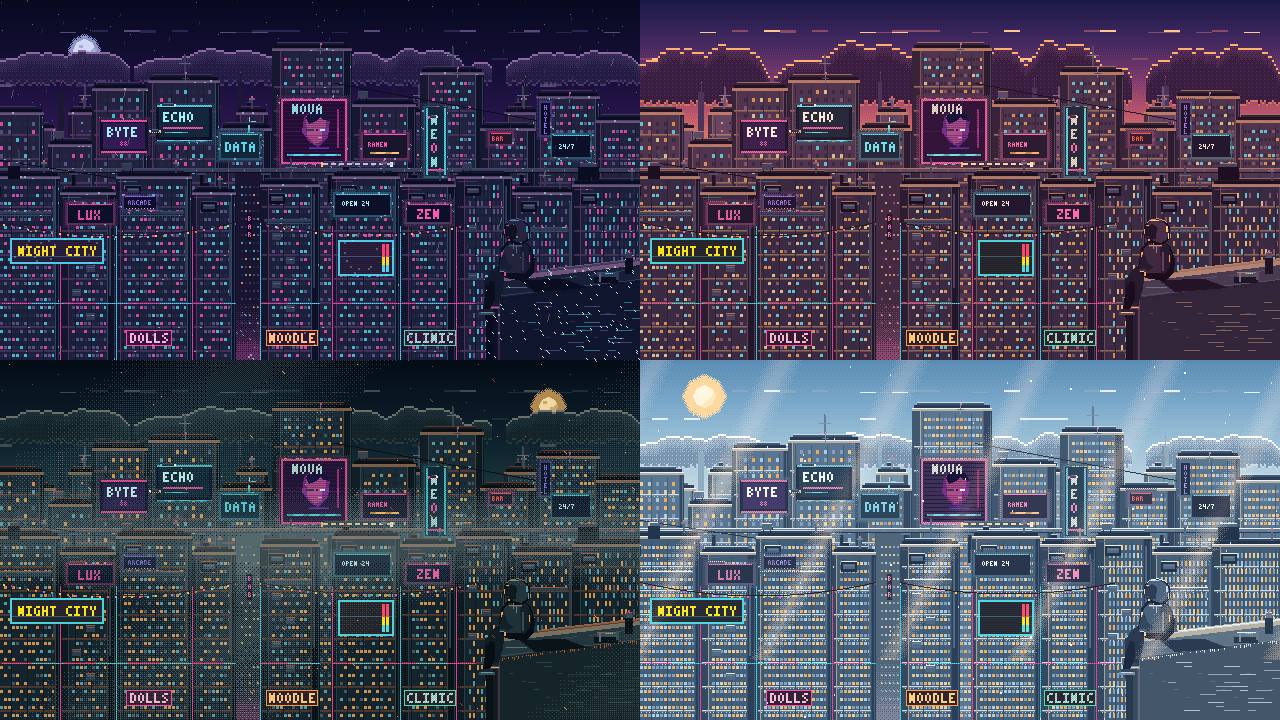
\includegraphics[width=0.96\textwidth]{figures/four_seasons_design.png}
\caption{四季动态夜城设计效果}\label{fig:seasons}
\end{figure}

\subsection{应用领域}
作品面向需要长期、离线展示音画内容的场合：
\begin{itemize}
\item \textbf{展厅与博物馆}：静态图片承担展品介绍与科普讲解，中文字幕补充说明，背景音乐营造氛围；
\item \textbf{商业空间与橱窗}：轮播产品图片，空闲时切换到动态夜城作为吸引视线的数字艺术背景；
\item \textbf{校园与公共信息屏}：轮播通知、安全提示等图片，内容更新只需替换 TF 卡素材；
\item \textbf{家居数字画框}：播放个人照片与音乐，四季场景提供随时间变化的装饰画面。
\end{itemize}
设备不依赖网络和上位机，准备好素材后由开发板独立运行；更换内容只需替换 TF 卡中的文件。

\subsection{主要技术特点}
\textbf{1. 纯 FPGA 实现的完整音画系统。}FAT32 根目录查找、BMP 与 WAV 解析、图像缩放、SDRAM 帧缓存、图层合成、音量处理和 HDMI 音视频封装全部由 FPGA 硬件逻辑完成，不使用软核处理器或外部主控。

\textbf{2. 多时钟域并行流水架构。}4 个 PLL 产生 50 MHz 卡访问、40 MHz 存储、25 MHz 画面合成、74.25 MHz 像素时钟及其 5 倍频串行时钟。各域以异步 FIFO、翻转令牌和请求／应答握手衔接，读卡、写缓存、扫描输出和音频播放并行推进、互不阻塞。

\textbf{3. 动态画面实时生成。}动态场景由像素坐标、季节色板和帧计数实时计算，不占用 TF 卡读取带宽；字幕、菜单、音频柱作为独立图层按坐标叠加，无需额外帧缓存。

\textbf{4. 资源高度集成。}在 19600 LUT 的器件中同时容纳基础功能、五类扩展和动态场景，LUT 利用率 91\%，32 Kb RAM 块与 PLL 全部用满，全部时钟域时序收敛。

\subsection{主要性能指标}
\begin{center}\small
\begin{tabular}{p{4.0cm}>{\raggedright\arraybackslash}p{9.5cm}}
\toprule
项目 & 指标\\\midrule
处理平台 & HX4S20C；EG4S20BG256；板载 50 MHz 时钟\\
视频输出 & HDMI，$1280\times720$@60 Hz，像素时钟 74.25 MHz；内部合成画布 $640\times360$\\
音频输出 & 48 kHz、16 位、双声道 PCM WAV，经 HDMI 传输；配套素材四首曲目可在菜单中选择\\
图片输入 & 24 位非压缩 BMP，根目录最多六张，宽高不超过 $1920\times1080$，运行时等比适配\\
图片缓存 & SDRAM 六帧缓存，共 5.27 MiB，切图无需重新读卡\\
自动轮播 & \tablegroup{3 / 5 / 15} 秒三档可选\\
动态场景 & 四季四景，1012 个城市图块，40 组季节色板，逐像素实时生成\\
交互与扩展 & 中文菜单、滚动字幕、淡入淡出转场、\tablegroup{亮度 / 对比度 / 音量}调节、64 柱幅度历史与街区音乐屏\\
资源占用 & LUT \tablegroup{17884 / 19600}（91\%）；SLICE \tablegroup{9192 / 9800}；PLL \tablegroup{4 / 4}\\
时序结果 & 全部时钟域 setup 与 hold 余量均为正，setup 最差余量 $+0.357$ ns，无时序违例\\
\bottomrule
\end{tabular}
\end{center}

\subsection{主要创新点}
\textbf{1. 一城四季的实时数字艺术。}作品没有把动画做成视频文件，而是把城市拆分为 $8\times8$ 像素图块，由 FPGA 按坐标查表并叠加实时天气与灯光。1012 个去重图块按实际颜色数分级编码：143 个只需 1 bit／像素，369 个使用 2 bit／像素，其余 500 个使用 4 bit／像素，比全部采用 4 bit 编码节省约 29\% 的图块存储。整座城市的图块与映射数据合计约 0.24 Mbit，而四张 $640\times360$ 真彩静图需要约 22.1 Mbit，相差 90 倍以上；若以 30 帧／秒视频播放同等画面，10 秒即需约 1.66 Gbit。实时生成使四季场景在不占用读卡带宽的情况下持续运动。

\textbf{2. 真实音频驱动的双层视觉反馈。}主画面 64 柱幅度历史和夜城街区广告屏的 12 柱音乐屏都直接取自播放链路中经音量处理后的 PCM 样本。作品展示随时间滚动的幅度包络，没有采用频谱：观众不需要音频知识，就能看到鼓点和旋律起伏与柱形同步跳动；调节音量时，声音与柱高一起变化。幅度计算只需累加与移位，节省出的乘法器和存储资源用于实现动态场景。

\textbf{3. 完整帧呈现的多媒体融合。}六帧 SDRAM 缓存、运行时等比缩放、淡入淡出转场、中文菜单与滚动字幕协同工作；切图时只有完整写入的画面才会被发布显示，HDMI 扫描和音乐播放全程不中断。静图展示与动态场景共用同一套音画输出和交互控制，切换模式时只改变显示内容，不需要重新加载系统。

\subsection{设计流程}
设计按“基础链路优先、功能逐级集成”的原则推进：首先完成需求分解与板卡接口确认，建立 TF 读图、SDRAM 缓存和 HDMI 音画输出的基础链路；随后在统一的时钟与资源预算内逐步加入缩放、六帧缓存、图层、字幕、菜单和动态场景；每项功能经模块仿真、布局布线和上板验证后再进入下一轮集成，最终以同一镜像固化并验证上电自启动。图\ref{fig:workflow}概括该过程。

\begin{figure}[H]\centering
\begin{tikzpicture}[node distance=7mm, box/.style={draw,rounded corners,align=center,minimum width=2.7cm,minimum height=0.8cm,fill=blue!5}, arr/.style={-{Latex},thick}]
\node[box] (a) {需求与接口}; \node[box,right=of a] (b) {音画基础链路}; \node[box,right=of b] (c) {缓存与图层};
\node[box,below=of c] (d) {动态场景与交互}; \node[box,left=of d] (e) {仿真与布局布线}; \node[box,left=of e] (f) {固化与实物验证};
\draw[arr](a)--(b); \draw[arr](b)--(c); \draw[arr](c)--(d); \draw[arr](d)--(e); \draw[arr](e)--(f);
\draw[arr,dashed](e.south)--++(0,-0.45)-|node[pos=0.25,below,font=\small]{迭代优化}(d.south);
\end{tikzpicture}
\caption{作品设计与验证流程}\label{fig:workflow}
\end{figure}

\section{系统组成及功能说明}

\subsection{整体介绍}
系统以 EG4S20 FPGA 为核心，构建“素材输入—处理—缓存—合成—输出”的全硬件音画链路，由输入与控制、图片处理、音频处理、动态场景、帧缓存和 HDMI 输出六个子系统组成（图\ref{fig:architecture}）。

\begin{enumerate}
\item \textbf{输入与控制子系统}：作为“交互入口”，对按键和拨码开关做同步与消抖，按当前模式将事件路由到菜单、切图或场景控制。
\item \textbf{图片处理子系统}：作为“图像入口”，从 TF 卡读取 BMP 文件，解析文件头，完成等比双线性缩放与居中补黑。
\item \textbf{音频处理子系统}：作为“声音入口”，解析 WAV 文件得到 48 kHz 立体声 PCM，完成音量渐变，并同时送往 HDMI 音频通道和可视化逻辑。
\item \textbf{帧缓存子系统}：作为“数据中转站”，以 SDRAM 六帧缓存解耦读卡速率与显示速率，配合受控刷新调度保证读写连续。
\item \textbf{动态场景子系统}：作为“数字艺术引擎”，根据像素坐标、季节和时间实时生成四季夜城画面。
\item \textbf{图层合成与 HDMI 输出子系统}：作为“输出终端”，叠加转场、字幕、音频柱和菜单，将 $640\times360$ 画布倍扫为 720p60，并与音频一起封装为 HDMI 信号。
\end{enumerate}

\begin{figure}[H]\centering
\begin{tikzpicture}[x=1cm,y=1cm, node/.style={draw,rounded corners,align=center,fill=blue!5,minimum width=2.4cm,minimum height=0.75cm}, arrow/.style={-{Latex},thick}]
\node[node] (tf) at (0,3) {TF 卡\\图片与音乐};
\node[node] (bmp) at (3.5,4) {BMP 解析\\等比缩放};
\node[node] (wav) at (3.5,2) {WAV 解码\\PCM 音量};
\node[node] (mem) at (7,4) {SDRAM\\六帧缓存};
\node[node] (scene) at (7,2) {四季场景\\实时生成};
\node[node] (mix) at (10.5,3) {画面合成\\字幕、菜单、音频柱};
\node[node] (out) at (10.5,0.8) {HDMI 输出\\显示器与音响};
\node[node] (ctl) at (3.5,0) {按键／拨码\\统一控制};
\draw[arrow](tf)--(bmp); \draw[arrow](tf)--(wav); \draw[arrow](bmp)--(mem); \draw[arrow](mem)--(mix); \draw[arrow](scene)--(mix); \draw[arrow](mix)--(out); \draw[arrow](wav.south)--++(0,-0.45)-|(out.west); \draw[arrow](wav)--(scene); \draw[arrow](ctl)--(scene); \draw[arrow](ctl)--(wav);
\end{tikzpicture}
\caption{系统功能与数据流框图}\label{fig:architecture}
\end{figure}

图像通路以完整帧为单位组织：读取文件头后确定缩放几何，缩放后的画布写入对应的 SDRAM 缓存区，只有整帧写完的画面才会被发布显示。显示一侧按固定视频时序持续扫描，HDMI 时钟从不因读卡而暂停。音频通路独立维持 48 kHz 样本节拍，切图和场景切换不会打断背景音乐。PC 仅在素材准备和设计编译阶段使用，设备运行时的图像缩放、场景渲染和音频处理全部由 FPGA 完成。

\subsection{硬件系统介绍}
\subsubsection{硬件整体介绍}
系统硬件采用“核心处理—存储—外设接口”三层架构：核心层为 EG4S20BG256 FPGA 及板载 50 MHz 时钟 [3]；存储层包括器件合封的 $2\mathrm{M}\times32$ 位 SDRAM 和保存配置镜像的 SPI Flash；外设层包括 TF 卡、HDMI 接口、4 个按键和 4 个拨码开关。HDMI 接口同时送出画面与声音，显示器或音响即可直接播放。

\begin{center}\small
\begin{tabular}{p{3.0cm}p{4.2cm}p{6.2cm}}
\toprule
部件 & 连接与接口 & 作用\\\midrule
FPGA & EG4S20BG256，19600 LUT & 并行处理、缓存控制、图层合成、音画输出\\
TF 卡 & 板载卡槽，SPI 模式 & 保存 BMP 图片和 WAV 音乐文件\\
合封 SDRAM & $2\mathrm{M}\times32$ 位，8 MiB & 六帧图像缓存，解耦读卡与扫描\\
配置 Flash & 板载 SPI Flash & 保存固化镜像，上电自动加载\\
HDMI 接口 & 3 对 TMDS 数据＋1 对时钟 & 输出 720p60 视频与 48 kHz 音频\\
按键与拨码 & KEY1--KEY4，SW1--SW3 & 复位、菜单、切图、轮播与场景控制\\
\bottomrule
\end{tabular}
\end{center}
使用时在断电状态插入已准备素材的 TF 卡，连接 HDMI 显示器后上电即可运行，正常展示无需连接电脑。

\subsubsection{HDMI 接口电路}
HDMI 是本系统唯一的音画输出通道，也是板级最高速的接口：720p60 下每对 TMDS 数据线的串行速率达 742.5 Mbit/s。图\ref{fig:sch-hdmi}截取自开发板原理图的 HDMI 部分。FPGA 输出的 3 对数据差分和 1 对时钟差分先经 0.01 µF 电容交流耦合，再经 AZ1045-04F 四通道 ESD 保护阵列（U133、U135）接入 HDMI-019S 连接器 J7；DDC 的 SCL／SDA 由 TXB0104 双向电平转换器（U132）在 FPGA 侧与 HDMI 5 V 侧之间转换，HPD 与 CEC 由 U137 提供静电保护，连接器 5 V 供电经二极管 D4 隔离倒灌。

\begin{figure}[H]\centering
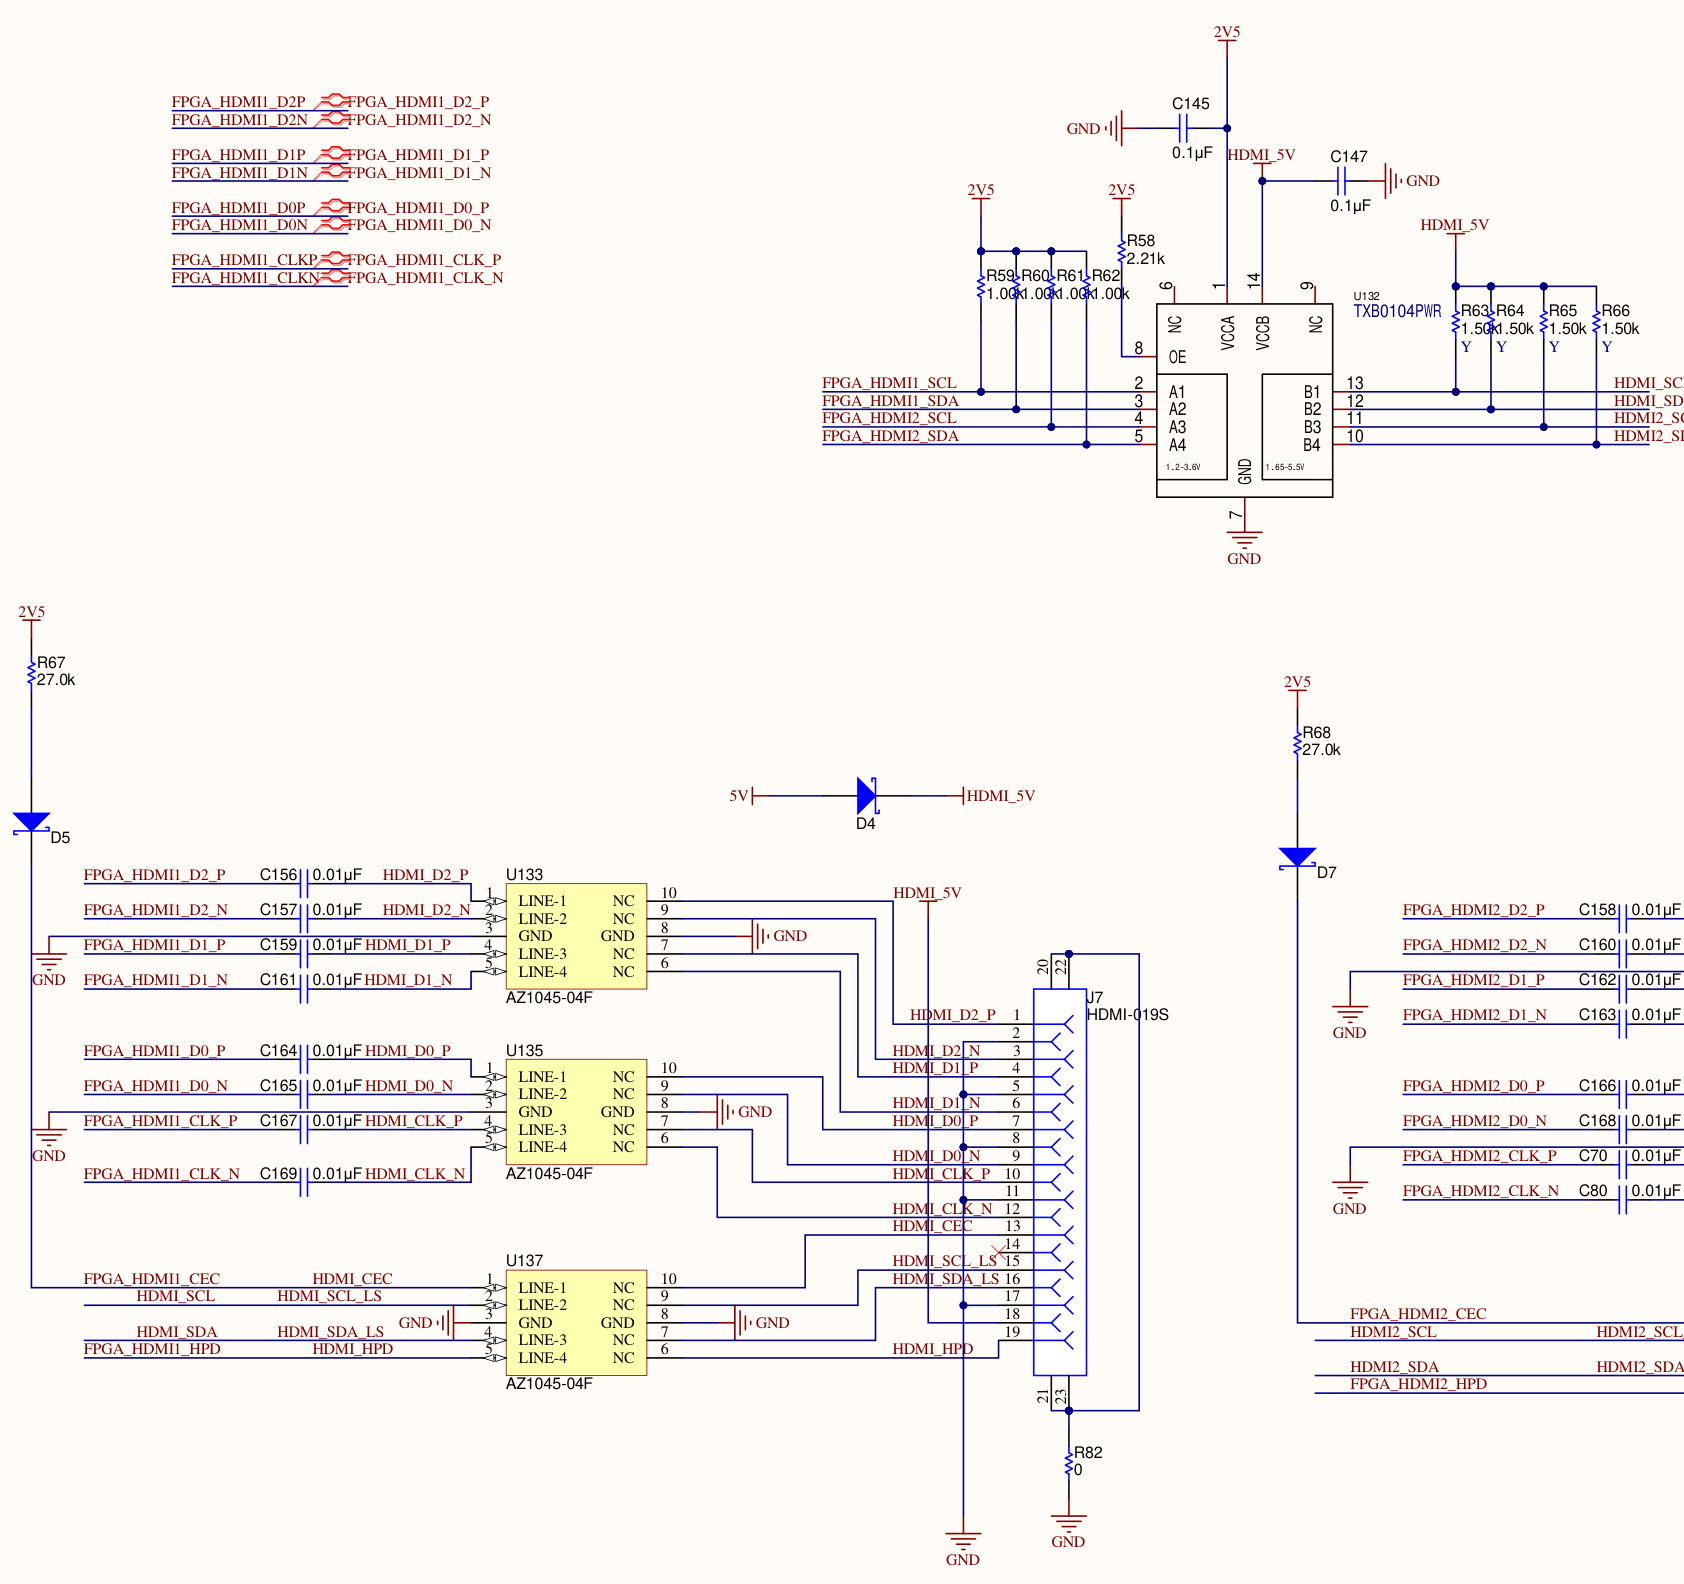
\includegraphics[width=0.88\textwidth]{figures/sch_hdmi.png}
\caption{HDMI 接口电路（截取自开发板原理图）}\label{fig:sch-hdmi}
\end{figure}

工程约束将 TMDS 通道配置为 FPGA 的 LVDS33 差分输出，由片内 10:1 串行化逻辑驱动；DDC 引脚配置为带上拉的 LVCMOS33。系统使用的主要外设引脚如下表所示。

\begin{center}\small
\begin{tabular}{p{4.4cm}C{2.1cm}C{2.1cm}>{\raggedright\arraybackslash}p{4.5cm}}
\toprule
信号 & 引脚 & IO 标准 & 功能\\\midrule
clk & R7 & LVCMOS33 & 板载 50 MHz 系统时钟\\
HDMI\_CLK\_P & C3 & LVDS33 & TMDS 时钟通道\\
\tablegroup{HDMI\_D0\_P / D1\_P / D2\_P} & \tablegroup{G5 / F1 / E1} & LVDS33 & TMDS 数据通道 \tablegroup{0 / 1 / 2}\\
\tablegroup{HDMI\_DDC\_SCL / SDA} & \tablegroup{P2 / R2} & LVCMOS33 & DDC 总线，内部上拉\\
\tablegroup{sd\_ncs / sd\_dclk} & \tablegroup{A12 / A14} & LVCMOS33 & TF 卡 SPI 片选与时钟\\
\tablegroup{sd\_mosi / sd\_miso} & \tablegroup{A13 / B14} & LVCMOS33 & TF 卡 SPI 数据输出与输入\\
\tablegroup{rst\_n / key1 / key3 / key2} & \tablegroup{A2 / B2 / B1 / C1} & LVCMOS33 & KEY1 复位，KEY2 确认，\tablegroup{KEY3 / KEY4} 方向\\
\tablegroup{sw[0] / [1] / [2]} & \tablegroup{C8 / C7 / C6} & LVCMOS33 & SW1 轮播，SW2 菜单，SW3 动态场景\\
\bottomrule
\end{tabular}
\end{center}

\subsubsection{时钟系统}
EG4S20 共有 4 个 PLL，本设计全部使用。板载 50 MHz 时钟输入后分为三路：\texttt{sys\_pll} 产生 50 MHz 卡访问时钟、40 MHz 存储时钟及 SDRAM 相移时钟；\texttt{video\_pll} 产生 25 MHz 画面合成时钟；\texttt{hd720\_ref27} 先生成 27 MHz 参考，再由 \texttt{hd720\_video\_pll} 级联产生 74.25 MHz 像素时钟和约 371 MHz 的五倍频串行时钟。两级级联让 720p 标准像素频率可以精确得到。

\begin{figure}[H]\centering
\begin{tikzpicture}[node distance=5mm and 9mm,box/.style={draw,rounded corners,align=center,minimum width=2.5cm,minimum height=0.75cm,fill=blue!5},clk/.style={draw,align=left,minimum width=4.6cm,minimum height=0.6cm,fill=orange!8,font=\small},arr/.style={-{Latex},thick}]
\node[box] (osc) {板载晶振\\50 MHz};
\node[box,right=of osc,yshift=1.6cm] (p1) {sys\_pll};
\node[box,right=of osc] (p2) {video\_pll};
\node[box,right=of osc,yshift=-1.6cm] (p3) {hd720\_ref27\\27 MHz};
\node[box,right=of p3] (p4) {hd720\_video\_pll};
\node[clk,right=of p1,xshift=2.4cm,yshift=0.35cm] (c1) {50 MHz：TF 访问、BMP／WAV 解析};
\node[clk,below=1mm of c1] (c2) {40 MHz：SDRAM 控制与刷新};
\node[clk,right=of p2,xshift=2.4cm] (c3) {25 MHz：画面合成、场景、菜单};
\node[clk,right=of p4,yshift=0.35cm] (c4) {74.25 MHz：720p 像素扫描};
\node[clk,below=1mm of c4] (c5) {约 371 MHz：TMDS 串行化};
\draw[arr](osc)--(p2); \draw[arr](osc.north)|-(p1); \draw[arr](osc.south)|-(p3); \draw[arr](p3)--(p4);
\draw[arr](p1.east)--++(0.4,0)|-(c1.west); \draw[arr](p1.east)--++(0.4,0)|-(c2.west); \draw[arr](p2)--(c3);
\draw[arr](p4.east)--++(0.3,0)|-(c4.west); \draw[arr](p4.east)--++(0.3,0)|-(c5.west);
\end{tikzpicture}
\caption{系统时钟树}\label{fig:clock}
\end{figure}

各时钟域的时序收敛情况如下表，数据取自最终镜像的布局布线时序报告。

\begin{center}\small
\begin{tabular}{p{3.6cm}p{2.0cm}p{2.6cm}p{2.3cm}p{2.3cm}}
\toprule
时钟域 & 约束频率 & 可达频率 & setup 余量 & hold 余量\\\midrule
TF 访问 & 50 MHz & 55.6 MHz & +0.868 ns & +0.027 ns\\
画面合成 & 25 MHz & 28.7 MHz & +1.658 ns & +0.027 ns\\
SDRAM 存储 & 40 MHz & 45.5 MHz & +1.456 ns & +0.035 ns\\
720p 像素 & 74.25 MHz & 105.2 MHz & +3.960 ns & +0.004 ns\\
TMDS 串行 & 371.3 MHz & 497.3 MHz & +0.682 ns & +0.162 ns\\
\bottomrule
\end{tabular}
\end{center}

\subsection{FPGA 逻辑系统介绍}
\subsubsection{逻辑系统整体介绍}
逻辑设计按数据来源和时钟职责分层。顶层 \texttt{top} 负责时钟、复位与各子系统互连；素材层 \texttt{sd\_card\_bmp} 统一调度 TF 卡上的图片和音乐；存储层 \texttt{frame\_read\_write} 管理写 FIFO、读 FIFO 与 SDRAM；显示层包括转场、场景、图层叠加和 720p 扫描输出；控制层 \texttt{player\_menu\_control} 处理按键事件与菜单参数。图\ref{fig:hierarchy}给出主要模块的层次关系。

\begin{figure}[H]\centering
\begin{tikzpicture}[font=\small,
 top/.style={draw,thick,rounded corners,fill=blue!12,minimum width=3cm,minimum height=0.7cm},
 grp/.style={draw,rounded corners,fill=blue!5,align=center,minimum width=2.6cm,minimum height=0.65cm},
 leaf/.style={draw,align=left,fill=white,font=\scriptsize\ttfamily,inner sep=2pt,text width=2.55cm},
 arr/.style={-{Latex},semithick}]
\node[top] (t) at (0,0) {\texttt{top}};
\node[grp] (g1) at (-6,-1.4) {素材层};
\node[grp] (g2) at (-3,-1.4) {存储层};
\node[grp] (g3) at (0,-1.4) {显示层};
\node[grp] (g4) at (3,-1.4) {音频层};
\node[grp] (g5) at (6,-1.4) {控制层};
\foreach \g in {g1,g2,g3,g4,g5} \draw[arr](t.south)--(\g.north);
\node[leaf,below=3mm of g1] {sd\_card\_bmp\\ sd\_card\_top\\ bmp\_read\\ stream\_scaler\\ music\_track\\ \quad\_player\\ wav\_pcm\_decode};
\node[leaf,below=3mm of g2] {frame\_read\_write\\ wfifo／rfifo\\ sdram\\ sdram\_refresh\\ \quad\_control};
\node[leaf,below=3mm of g3] {image\_fade\\ \quad\_transition\\ night\_city\_scene\\ video\_adjust\_osd\\ player\_menu\\ \quad\_overlay\\ hd720\_composite\\ \quad\_scanout};
\node[leaf,below=3mm of g4] {music\_pcm\_output\\ pcm\_volume\_slew\\ music\_rhythm\\ \quad\_overlay\\ audio\_arc\\ \quad\_calculate\\ hdmi\_1\_4b\_tx\\ hd720\_phy};
\node[leaf,below=3mm of g5] {player\_menu\\ \quad\_control\\ player\_scene\\ \quad\_control\\ player\_scene\\ \quad\_restore};
\end{tikzpicture}
\caption{FPGA 逻辑模块层次}\label{fig:hierarchy}
\end{figure}

图片与音乐素材在电脑端按规定格式准备；运行时的文件解析、缩放、缓存、合成、显示和声音播放全部在 FPGA 内完成。场景图块、字库和字幕在构建时打包为片上 ROM，天气、灯光、菜单和音频柱在运行时由逻辑实时生成。设计使用了赛题支持的厂商 SDRAM、FIFO 与 HDMI 基础 IP，以及开源流式视频缩放核 [6]；素材调度、六帧缓存组织、刷新调度、图层合成、中文交互、音频可视化和四季动态场景等业务逻辑均为本作品自主设计 [7]。

\subsubsection{跨时钟域设计}
系统共有 5 个主要工作时钟域，模块间的交互遵循三条规则：
\begin{itemize}
\item \textbf{单比特状态}：使用两到三级 \texttt{async\_reg} 同步器链，降低亚稳态向后级传播的概率；
\item \textbf{多比特数据}（缓存编号、曲目标题、帧标签等）：采用“数据保持＋翻转令牌＋应答”握手。发送方先锁存数据再翻转令牌，接收方同步令牌后才采样数据，发送方在收到应答之前保持数据不变，避免多位数据逐位跨域产生混合值；
\item \textbf{连续数据流}（像素、PCM 样本）：使用格雷码指针的异步 FIFO。
\end{itemize}

\begin{figure}[H]\centering
\begin{tikzpicture}[font=\small,dom/.style={draw,thick,rounded corners,fill=blue!5,align=center,minimum width=2.6cm,minimum height=1.2cm},lab/.style={font=\scriptsize,align=center,fill=white,inner sep=1pt},arr/.style={-{Latex},thick}]
\node[dom] (sd) at (0,2) {TF 访问域\\50 MHz};
\node[dom] (mem) at (5,2) {存储域\\40 MHz};
\node[dom] (vid) at (5,-0.5) {画面合成域\\25 MHz};
\node[dom] (pix) at (10,-0.5) {像素域\\74.25 MHz};
\node[dom] (ser) at (10,2) {串行域\\$5\times$像素};
\draw[arr](sd)--node[lab]{写 FIFO\\像素流}(mem);
\draw[arr](mem)--node[lab]{读 FIFO\\像素流}(vid);
\draw[arr,dashed](sd.south)|-node[lab,pos=0.75]{缓存编号\\令牌握手}(vid.west);
\draw[arr,dashed]([xshift=-6mm]sd.south)--++(0,-3.4)-|node[lab,pos=0.25]{PCM 样本 FIFO}([xshift=-6mm]vid.south);
\draw[arr](vid)--node[lab]{像素 FIFO\\帧标签}(pix);
\draw[arr](pix)--node[lab]{10 bit\\TMDS 码}(ser);
\draw[arr,dashed](pix.south)--++(0,-0.6)-|node[lab,pos=0.25]{帧完成令牌}(vid.south);
\end{tikzpicture}
\caption{主要时钟域及跨域方式（实线为数据流，虚线为控制握手）}\label{fig:cdc}
\end{figure}

复位同样按域处理：全局复位由按键 KEY1 和 PLL 锁定信号共同产生，各时钟域在本域时钟下经三级同步后释放，保证复位撤销沿与本域时钟对齐。

\subsubsection{图片读取与等比缩放模块}
\paragraph{模块功能。}\texttt{sd\_card\_bmp} 是素材服务的顶层：它在 TF 卡初始化完成后按图片清单依次加载六幅 BMP，同时为音乐播放器分配扇区读取机会；\texttt{bmp\_read} 解析文件头、按行读取像素并送入缩放核，输出的画布像素经写 FIFO 进入 SDRAM。底层 SPI 控制器在初始化阶段以低速工作，进入数据阶段后切换到 $50/4=12.5$ MHz 高速时钟。

\begin{center}\small
\begin{tabular}{>{\raggedright\arraybackslash\ttfamily\footnotesize}p{6.0cm}C{1.0cm}C{1.6cm}>{\raggedright\arraybackslash}p{4.7cm}}
\toprule
信号名 & 位宽 & 方向 & 功能描述\\\midrule
\tablegroup{clk / rst} & 1 & Input & 50 MHz 卡访问时钟与复位\\
\tablegroup{key\_next / nav\_toggle} & 1 & Input & 切图请求，翻转令牌形式\\
picture\_select\_index & 3 & Input & 菜单指定的目标图片编号\\
\tablegroup{auto\_enable / auto\_toggle} & 1 & Input & 自动轮播使能与到期事件\\
write\_buf\_idx & 3 & Output & 当前写入的缓存编号（0--5）\\
disp\_buf\_idx & 3 & Output & 已完成、可供显示的缓存编号\\
frame\_ready\_toggle & 1 & Output & 新帧就绪令牌，跨域通知显示侧\\
frame\_presented\_toggle & 1 & Input & 显示侧呈现应答\\
\tablegroup{write\_req / write\_req\_ack} & 1 & \tablegroup{Out / In} & SDRAM 帧写请求握手\\
\tablegroup{write\_en / write\_data} & \tablegroup{1 / 32} & Output & 缩放后像素写入写 FIFO\\
\tablegroup{music\_valid / music\_sample} & \tablegroup{1 / 32} & Output & 解码后的左右声道 PCM 样本\\
track\_select\_index & 3 & Input & 菜单选曲编号\\
track\_titles & 1240 & Output & 曲目标题字符串，用于菜单显示\\
\tablegroup{SD\_nCS / SD\_DCLK / SD\_MOSI} & 1 & Output & SPI 片选、时钟、数据输出\\
SD\_MISO & 1 & Input & SPI 数据输入\\
\bottomrule
\end{tabular}
\end{center}

\paragraph{BMP 文件解析。}读取逻辑首先检查文件标识、像素数据偏移、宽高、位深与压缩类型，再按行访问像素。BMP 每行按 4 字节对齐，对宽度为 $W$ 的 RGB24 图像，一行在文件中的字节跨度为
\begin{equation}
S_{\mathrm{row}}=4\left\lceil\frac{3W}{4}\right\rceil ,
\end{equation}
其中 $3W$ 为有效像素字节，余下部分为行尾填充，解析时跳过。BMP 高度的符号决定行顺序，逻辑据此选择逐行地址方向；B、G、R 字节重排后进入 RGB 通路。

\paragraph{等比缩放和居中补黑。}设源图尺寸为 $W_s\times H_s$，目标画布为 $W_d\times H_d$，等比适配的缩放系数与内容区尺寸为
\begin{equation}
s=\min\left(\frac{W_d}{W_s},\frac{H_d}{H_s}\right),\quad
W_o=\lfloor sW_s\rfloor,\quad H_o=\lfloor sH_s\rfloor .
\end{equation}
内容区以外居中填黑。以 $640\times480$ 输入为例，$s=0.75$，内容区为 $480\times360$，左右各留 80 个画布像素；输出倍扫后对应 $960\times720$ 内容区。由于缩放参数在运行时根据文件头计算，同一画布可以正确呈现 4:3、16:9 等不同比例的图片，素材无需在电脑上预先统一尺寸。

\paragraph{双线性插值。}输出像素映射到源图中的小数坐标 $(x_s,y_s)$，令左上邻点为 $(i,j)$，水平与垂直小数部分为 $a,b$，则
\begin{align}
P(x_s,y_s)={}&(1-a)(1-b)P_{i,j}+a(1-b)P_{i+1,j}\nonumber\\
 &+(1-a)bP_{i,j+1}+abP_{i+1,j+1}.
\end{align}
R、G、B 分量分别计算，定点精度与边界处理由流式缩放核实现。文件行读取、缩放核的有效／就绪握手和写 FIFO 背压构成连续流水，缩放核内部用行缓存保存相邻两行，无需整帧暂存源图。

\begin{figure}[H]\centering
\begin{tikzpicture}[node distance=6mm,box/.style={draw,rounded corners,align=center,minimum width=2.3cm,minimum height=0.8cm,fill=blue!5},arr/.style={-{Latex},thick}]
\node[box] (a) {TF 扇区读取}; \node[box,right=of a] (b) {BMP 头与行解析}; \node[box,right=of b] (c) {等比几何};
\node[box,below=of c] (d) {双线性缩放}; \node[box,left=of d] (e) {补黑与写 FIFO}; \node[box,left=of e] (f) {SDRAM 缓存};
\draw[arr](a)--(b); \draw[arr](b)--(c); \draw[arr](c)--(d); \draw[arr](d)--(e); \draw[arr](e)--(f);
\end{tikzpicture}
\caption{图片加载和缩放数据流}\label{fig:image-flow}
\end{figure}

\paragraph{卡访问仲裁。}图片与音乐共享同一张 TF 卡。扇区仲裁器 \texttt{sd\_sector\_arbiter} 在图片加载和音乐缓存之间分配读取机会：音乐 FIFO 低于水位时发出紧急请求，优先获得扇区，保证切图或启动加载期间背景音乐不断流。顺序扇区复用连续读会话，地址跳转时先结束旧会话再建立新访问。

\subsubsection{SDRAM 六帧缓存与刷新调度模块}
\paragraph{模块功能。}\texttt{frame\_read\_write} 将写入侧（50 MHz 素材像素流）、存储侧（40 MHz SDRAM 控制器）和读出侧（25 MHz 显示扫描）连接起来：写 FIFO 吸收缩放核输出的突发，读 FIFO 为显示扫描提前预取，SDRAM 以 256 字突发进行读写。外部刷新控制器 \texttt{sdram\_refresh\_control} 在存储域内统一调度刷新，保证刷新与读写事务互不重叠。

\begin{center}\small
\begin{tabular}{>{\raggedright\arraybackslash\ttfamily\footnotesize}p{6.0cm}C{1.0cm}C{1.6cm}>{\raggedright\arraybackslash}p{4.7cm}}
\toprule
信号名 & 位宽 & 方向 & 功能描述\\\midrule
mem\_clk & 1 & Input & 40 MHz 存储时钟\\
\tablegroup{write\_clk / read\_clk} & 1 & Input & 写入侧与读出侧时钟\\
\tablegroup{write\_req / write\_req\_ack} & 1 & \tablegroup{In / Out} & 帧写请求与应答，请求保持至应答\\
write\_addr\_index & 3 & Input & 写入目标缓存编号\\
\tablegroup{write\_en / write\_data} & \tablegroup{1 / 32} & Input & 写入像素，每像素一个 32 位字\\
write\_finish & 1 & Output & 整帧写入完成\\
\tablegroup{read\_req / read\_req\_ack} & 1 & \tablegroup{In / Out} & 帧读请求与应答\\
read\_addr\_index & 3 & Input & 读出缓存编号\\
\tablegroup{read\_en / read\_data} & \tablegroup{1 / 32} & \tablegroup{In / Out} & 显示侧逐像素读取\\
\tablegroup{read\_empty / read\_valid} & 1 & Output & 读 FIFO 空标志与数据有效\\
\tablegroup{App\_wr\_en / App\_wr\_addr} & \tablegroup{1 / 21} & Output & 送往 SDRAM 控制器的写命令与字地址\\
\tablegroup{App\_rd\_en / App\_rd\_addr} & \tablegroup{1 / 21} & Output & 送往 SDRAM 控制器的读命令与字地址\\
\tablegroup{Sdr\_rd\_en / Sdr\_rd\_dout} & \tablegroup{1 / 32} & Input & SDRAM 读返回数据\\
managed\_refresh\_req & 1 & Output & 受控刷新请求\\
\bottomrule
\end{tabular}
\end{center}

\paragraph{六帧缓存组织。}每帧按 $640\times360$ 个 32 位字分配，六帧总容量为
\begin{equation}
6\times640\times360\times4=5\,529\,600\ \mathrm{B}\approx5.27\ \mathrm{MiB},
\end{equation}
占 8 MiB SDRAM 的 65.9\%。六个区域的起始字地址依次为 0、230400、460800、691200、921600 和 1152000。启动阶段六幅图片依次写入各自区域，之后切图只需改变读出缓存编号，无需再次读卡和缩放，切换响应只受转场时长限制。

\begin{figure}[H]\centering
\begin{tikzpicture}[font=\small,cell/.style={draw,minimum width=1.85cm,minimum height=0.8cm,align=center,fill=blue!5},free/.style={draw,minimum width=3.3cm,minimum height=0.8cm,align=center,fill=gray!10}]
\node[cell] (b0) at (0,0) {帧 0\\腕表};
\node[cell,right=0mm of b0] (b1) {帧 1\\饮品};
\node[cell,right=0mm of b1] (b2) {帧 2\\芯片};
\node[cell,right=0mm of b2] (b3) {帧 3\\暴雨提示};
\node[cell,right=0mm of b3] (b4) {帧 4\\车道提示};
\node[cell,right=0mm of b4] (b5) {帧 5\\课堂};
\node[free,right=0mm of b5] {未使用\\2.73 MiB};
\foreach \n/\a in {b0/0,b1/230400,b2/460800,b3/691200,b4/921600,b5/1152000} \node[font=\scriptsize,below=1mm of \n.south west,anchor=north west] {\a};
\end{tikzpicture}
\caption{SDRAM 六帧缓存地址分配（字地址）}\label{fig:sdram-map}
\end{figure}

\paragraph{受控刷新状态机。}SDRAM 必须周期性刷新，若刷新命令插入正在进行的突发读写，将破坏读写时序。为此，刷新控制器在 40 MHz 存储域内以五状态机统一调度（图\ref{fig:refresh-fsm}）：刷新年龄达到 800 个周期（20 µs）后进入 DRAIN，暂停发起新突发，等待在途事务和返回数据全部排空；连续 4 拍空闲后发出刷新请求，依次观察控制器刷新忙信号的上升和下降，再经 4 拍稳定后恢复 RUN。刷新间隔保证在 1250 个周期（31.25 µs）以内，满足 SDRAM 刷新要求。

\begin{figure}[H]\centering
\begin{tikzpicture}[font=\small,st/.style={draw,thick,circle,minimum size=1.5cm,align=center,fill=blue!5,font=\scriptsize},arr/.style={-{Latex},thick},lab/.style={font=\scriptsize,align=center}]
\node[st] (run) at (0,0) {RUN};
\node[st] (drain) at (3.6,0) {DRAIN};
\node[st] (rise) at (7.2,0) {WAIT\\\_RISE};
\node[st] (low) at (7.2,-2.6) {WAIT\\\_LOW};
\node[st] (settle) at (3.6,-2.6) {SETTLE};
\draw[arr](run)--node[lab,above]{age $\ge$ 799}(drain);
\draw[arr](drain)--node[lab,above]{空闲 4 拍\\发 refresh\_req}(rise);
\draw[arr](rise)--node[lab,right]{ref\_busy=1}(low);
\draw[arr](low)--node[lab,below]{ref\_busy=0}(settle);
\draw[arr](settle)--node[lab,below left]{空闲 4 拍}(run);
\draw[arr](drain) to[loop above] node[lab,above]{未排空} (drain);
\end{tikzpicture}
\caption{SDRAM 受控刷新状态机}\label{fig:refresh-fsm}
\end{figure}

控制器同时维护在途读事务计数：发起读而未同时返回时加一，返回而未同时发起时减一。只有“无挂起读写、无有效返回、在途计数为零、控制器非忙”同时成立时，存储路径才判定为空闲。

\begin{lstlisting}[style=Verilog]
case ({app_read, sdr_read_valid})
  2'b10: if (outstanding >= 512) fault <= 1;
         else outstanding <= outstanding + 1'b1;
  2'b01: if (outstanding == 0) fault <= 1;
         else outstanding <= outstanding - 1'b1;
  default: outstanding <= outstanding;
endcase
\end{lstlisting}

\paragraph{完整帧呈现。}缓存编号从素材域发布到显示域时，加载侧先锁存目标编号，再翻转 \texttt{frame\_ready\_toggle}；显示侧同步令牌后读取稳定的编号，在帧边界完成切换后返回 \texttt{frame\_presented\_toggle}。只有整帧写入完成的缓存才会被发布，观众始终看到完整画面。

\subsubsection{音频播放与 HDMI 音频模块}
\paragraph{模块功能。}\texttt{music\_track\_player} 在 TF 卡根目录中定位四首曲目，\texttt{wav\_pcm\_decode} 解析 RIFF 结构并输出 16 位双声道样本；\texttt{music\_pcm\_output} 以 4096 样本 FIFO 缓冲数据，并按 48 kHz 节拍释放样本；\texttt{pcm\_volume\_slew} 完成音量调节；最终样本同时送往 HDMI 音频封装和两路可视化逻辑。

\begin{center}\small
\begin{tabular}{>{\raggedright\arraybackslash\ttfamily\footnotesize}p{6.0cm}C{1.0cm}C{1.6cm}>{\raggedright\arraybackslash}p{4.7cm}}
\toprule
信号名 & 位宽 & 方向 & 功能描述\\\midrule
\multicolumn{4}{l}{\textit{wav\_pcm\_decode}}\\
\tablegroup{byte\_valid / byte\_data} & \tablegroup{1 / 8} & Input & TF 扇区字节流\\
file\_size & 32 & Input & 文件长度，用于定位数据块\\
\tablegroup{sample\_valid / sample\_ready} & 1 & \tablegroup{Out / In} & 样本输出握手，支持背压\\
sample\_data & 32 & Output & 左右声道各 16 位 PCM\\
status & 4 & Output & 解码状态：\tablegroup{打开 / 播放 / 格式错误}\\\midrule
\multicolumn{4}{l}{\textit{pcm\_volume\_slew}}\\
volume\_level & 4 & Input & 菜单音量档位 0--10\\
\tablegroup{in\_valid / in\_left / in\_right} & \tablegroup{1 / 24} & Input & 输入样本\\
\tablegroup{out\_valid / out\_left / out\_right} & \tablegroup{1 / 24} & Output & 调整后的输出样本\\
\bottomrule
\end{tabular}
\end{center}

\paragraph{WAV 解码与选曲。}解码器按 RIFF 块结构逐块解析，跳过未知块并处理奇数长度填充，不依赖固定 44 字节文件头，兼容多种工具导出的 WAV。切换曲目时，播放器先清空旧曲数据，再为新曲建立播放状态，避免不同曲目的样本混合。播放 FIFO 预存 1024 个样本后才开始输出，吸收读卡间隙。

\paragraph{音量调节与平滑渐变。}音量共 11 档，档位 $v\in\{0,\dots,10\}$ 对应目标增益 $G_t=256v$。每个样本到来时，当前增益 $G$ 向目标值最多移动 10，输出为
\begin{equation}
y_{L,R}[n]=\frac{G[n]\cdot x_{L,R}[n]}{2560},\qquad
G[n]=G[n-1]+\operatorname{clip}_{[-10,\,10]}\big(G_t-G[n-1]\big).
\end{equation}
增益从 0 到满幅最多经过 256 个样本（约 5.3 ms），调节音量时不会出现“咔哒”声。乘除运算采用逐位迭代实现，每个样本约用 50 个时钟周期，不占用 DSP 资源。

\paragraph{HDMI 音频封装。}HDMI 将音频样本插入视频消隐期的数据岛传输，接收端需要依据 ACR（音频时钟恢复）参数还原采样率。按 HDMI 规范，ACR 参数满足
\begin{equation}
128 f_s = \frac{f_{\mathrm{TMDS}}\cdot N}{CTS},
\end{equation}
本设计取 48 kHz 的标准值 [8] $N=6144$，由 \texttt{audio\_arc\_calculate} 在像素时钟下对音频有效脉冲计数得到 CTS，并周期性发送 ACR 包。48 kHz、16 位双声道 PCM 的原始数据率为
\begin{equation}
R=48000\times2\times16=1\,536\,000\ \mathrm{bit/s}.
\end{equation}

\subsubsection{音频可视化模块}
\paragraph{设计思路。}音频可视化的目标是让观众“看见音乐”。作品采用幅度时间历史而非频谱分析：每根柱代表一小段时间内音乐的响度，柱形从右向左滚动，鼓点和旋律起伏一目了然，不熟悉音频知识的观众也能直接感受到画面与音乐同步；调节音量时柱高随声音一起变化，形成即时的互动反馈。幅度计算只需累加与移位，不需要 FFT 所需的大量乘法器和缓存，节省的资源用于实现四季动态场景。

\begin{center}\small
\begin{tabular}{>{\raggedright\arraybackslash\ttfamily\footnotesize}p{6.0cm}C{1.0cm}C{1.6cm}>{\raggedright\arraybackslash}p{4.7cm}}
\toprule
信号名 & 位宽 & 方向 & 功能描述\\\midrule
\tablegroup{clk / rst} & 1 & Input & 25 MHz 画面合成时钟与复位\\
audio\_valid & 1 & Input & 音量处理后的样本有效\\
\tablegroup{audio\_left / audio\_right} & 24 & Input & 左右声道 PCM 样本\\
enable & 1 & Input & 菜单中的可视化开关\\
\tablegroup{in\_hs / in\_vs / in\_de / in\_rgb} & \tablegroup{1 / 24} & Input & 上一图层的同步信号与像素\\
\tablegroup{out\_hs / out\_vs / out\_de / out\_rgb} & \tablegroup{1 / 24} & Output & 叠加柱形后的同步信号与像素\\
\bottomrule
\end{tabular}
\end{center}

\paragraph{幅度计算。}每 256 个立体声样本构成一个时间窗，窗内平均幅度为
\begin{equation}
E_k=\frac{1}{256}\sum_{n=256k}^{256k+255}\frac{|L[n]|+|R[n]|}{2}.
\end{equation}
为了让轻柔段落同样清晰可见，柱高 $h$ 采用分段压缩：$E_k$ 映射到 64 像素以内时线性显示，超过 64 后斜率降为 1/4，并限制在 2--112 范围内。64 个时间窗共覆盖 16384 个样本，即约 0.34 秒的音乐历史。

\paragraph{包络与峰值。}柱高更新采用“快升慢降”包络：新值高于当前柱时取二者平均快速上升，低于时每帧最多下降 3 像素；峰值标记缓慢回落。这样柱形既能紧跟节拍，又不会闪烁跳动。64 个历史值和包络存放在两块小容量同步 RAM 中，场消隐开始后用 128 个时钟周期（25 MHz 下 5.12 µs）统一刷新，完全在消隐期内完成，同一帧内柱状态保持一致。

\begin{lstlisting}[style=Verilog]
// fast attack, slow release; peak cap falls one pixel per frame
wire [6:0] next_height = target > old_height ? attack_sum[7:1] :
    (old_height > target + 7'd3 ? old_height - 7'd3 : target);
wire [6:0] next_peak = next_height >= old_peak ? next_height
                                               : old_peak - 1'b1;
\end{lstlisting}

\paragraph{像素覆盖。}画面宽度被划分为 64 个 10 像素槽，每槽 8 像素柱体加 2 像素间隔，颜色从青色经蓝色渐变到紫色。像素落在柱体或峰值标记范围内时输出柱色，其余位置透传下层像素，因此柱形可以叠加在静图和夜城之上，无需为它单独开辟帧缓存。

\paragraph{街区音乐屏。}夜城中第二块广告屏显示 12 根细柱：逻辑每帧提取一次当前 PCM 电平并保存 12 帧历史，新电平从一端写入、旧电平依次移动，颜色按高度分为青、黄、红三段。主画面柱与街区屏取自同一路最终 PCM 样本，粒度和尺寸不同，前者展示音乐的整体节奏，后者把音乐融入城市景观之中。

\begin{figure}[H]\centering
\begin{tikzpicture}[node distance=6mm,box/.style={draw,rounded corners,align=center,minimum width=2.45cm,minimum height=0.8cm,fill=blue!5},arr/.style={-{Latex},thick}]
\node[box] (a) {TF／WAV}; \node[box,right=of a] (b) {PCM 解码}; \node[box,right=of b] (c) {音量与渐变}; \node[box,right=of c] (d) {HDMI 音频};
\node[box,below=of c] (e) {幅度提取与历史}; \node[box,left=of e] (f) {64 柱／街区 12 柱};
\draw[arr](a)--(b); \draw[arr](b)--(c); \draw[arr](c)--(d); \draw[arr](c)--(e); \draw[arr](e)--(f);
\end{tikzpicture}
\caption{音频播放与可视化数据流}\label{fig:audio-flow}
\end{figure}

\subsubsection{四季动态夜城模块}
\paragraph{设计目标。}四季夜城需要在一块 FPGA 上同时满足三个要求：画面丰富、持续运动；四季风格统一、易于辨认；不占用 TF 卡带宽和 SDRAM 缓存。作品为此采用“静态图块＋季节色板＋实时动态层”的分层生成方案：城市的建筑轮廓和纹理只存一份，季节差异由色板和材质表表达，雨雪、云雾、灯光等运动元素由逻辑根据坐标与时间实时计算。

\begin{center}\small
\begin{tabular}{>{\raggedright\arraybackslash\ttfamily\footnotesize}p{6.0cm}C{1.0cm}C{1.6cm}>{\raggedright\arraybackslash}p{4.7cm}}
\toprule
信号名 & 位宽 & 方向 & 功能描述\\\midrule
\tablegroup{clk / rst} & 1 & Input & 25 MHz 画面合成时钟与复位\\
enable & 1 & Input & 动态场景使能（SW3）\\
scene\_select & 2 & Input & 季节编号：\tablegroup{雨夜 / 雷云 / 薄雾 / 飘雪}\\
audio\_valid & 1 & Input & 最终 PCM 样本有效\\
\tablegroup{audio\_left / audio\_right} & 24 & Input & 左右声道样本，驱动街区音乐屏\\
\tablegroup{in\_hs / in\_vs / in\_de / in\_rgb} & \tablegroup{1 / 24} & Input & 背景时序与静图像素\\
\tablegroup{out\_hs / out\_vs / out\_de / out\_rgb} & \tablegroup{1 / 24} & Output & 场景合成后的时序与像素\\
scene\_active & 1 & Output & 场景画面正在输出\\
\bottomrule
\end{tabular}
\end{center}

\paragraph{图块化城市。}$640\times360$ 场景画面被划分为 $80\times45=3600$ 个 $8\times8$ 图块。离线工具对整座城市去重后得到 1012 种不同图块，每个位置用一个 16 位映射字 \texttt{\{pal[5:0], tile[9:0]\}} 记录图块编号和所用的 40 组局部调色板之一。像素生成时，逻辑由坐标查映射表得到图块号，再查图块像素得到颜色槽，最后经调色板映射为材质码，材质码再按季节查表得到最终 RGB。

\paragraph{分级位宽无损编码。}不同图块需要的颜色数差别很大：天空和墙面往往只有一两种颜色，霓虹招牌则需要更多颜色。生成工具统计每个图块的实际颜色数，按需分配位宽，并将图块重新排序，使编码方式可由图块号直接判定：
\begin{center}\small
\begin{tabular}{p{3.0cm}p{2.2cm}p{2.6cm}p{5.0cm}}
\toprule
编码方式 & 图块数 & 每图块位数 & 适用内容\\\midrule
\tablegroup{1 bit / 像素} & 143 & 64 & 单色或双色墙面、天空\\
\tablegroup{2 bit / 像素} & 369 & 128 & 三至四色窗格、楼体细节\\
\tablegroup{4 bit / 像素} & 500 & 256 & 招牌、人物、霓虹光晕\\\midrule
合计 & 1012 & 184384 bit & 相比全部 4 bit 编码节省 28.8\%\\
\bottomrule
\end{tabular}
\end{center}
压缩图块的颜色槽经一张小映射表还原为 4 bit 索引，后级逻辑无需区分编码方式。节省出的片上存储用于容纳 214 个中文字幕字形，使场景和字幕能共存于同一器件。

\begin{lstlisting}[style=Verilog]
// tile id ranges select the encoding; one address adder per mode
wire tile_mono       = tile_id < 10'd143;   // 1 bit/pixel
wire tile_compressed = tile_id < 10'd512;   // 2 bit/pixel
wire [13:0] tile_address = tile_mono ?
    {2'b00,tile_id,2'b00} + logical_y[2:1] : tile_compressed ?
    {1'b0,tile_id,3'b000} - 14'd572 + logical_y[2:0] :
    {tile_id,4'b0000} - 14'd4668 + {logical_y[2:0],tile_x[2]};
\end{lstlisting}

\paragraph{季节材质与实时动态层。}季节 ROM 的每条记录为 \texttt{\{flags, R, G, B\}}，地址由季节号、特效位和材质码组成。同一材质码在四个季节对应不同颜色，特效位分别表示雨夜湿面反光、雷云闪电照亮、薄雾有序抖动和雪晨斜光混合；flags 选择霓虹的呼吸、闪烁、跑马和全息扫描方式。动态层包括天空渐变与云层、日月星辰、窗灯、街道车流、雨线雪粒、雾带、光束和闪电，以及人物的呼吸、衣角和冬季呼气，全部由坐标比较、计数器和少量查表实现。

\begin{figure}[H]\centering
\begin{tikzpicture}[node distance=5mm,box/.style={draw,align=center,minimum width=3.2cm,minimum height=0.75cm,fill=blue!5},arr/.style={-{Latex},thick}]
\node[box] (a) {共享城市图块／材质};
\node[box,right=of a] (b) {季节色板与场景身份};
\node[box,below=of a] (c) {天气、灯光与街区细节};
\node[box,below=of b] (d) {PCM 音频历史柱};
\node[box,below=of c,xshift=1.8cm] (e) {像素优先级合成与输出};
\draw[arr](a)--(e); \draw[arr](b)--(e); \draw[arr](c)--(e); \draw[arr](d)--(e);
\end{tikzpicture}
\caption{四季动态场景的组成}\label{fig:scene-layers}
\end{figure}

场景像素可抽象为
\begin{equation}
P_{\mathrm{scene}}(x,y,t)=\mathcal{C}\left(T(x,y),L_q, D_q(x,y,t),A(t)\right),
\end{equation}
其中 $T$ 为共享图块与材质，$L_q$ 为第 $q$ 个季节的色板，$D_q$ 为随时间变化的天气、灯光和细节，$A$ 为音频驱动的屏幕状态，$\mathcal{C}$ 按遮挡优先级选出最终像素。

\paragraph{三级像素流水。}由于片上 RAM 读出有一拍延迟，场景模块采用提前寻址的三级流水：映射表在像素到达前两拍寻址，图块数据提前一拍寻址，第三拍完成调色板、季节查表和动态层合成。同步信号随像素逐级延迟，保证图层边界与坐标严格对齐。复杂的边界判断与颜色选择分散到不同流水级，使 25 MHz 合成域留有 1.658 ns 的建立时间余量。

\paragraph{一城四季的视觉组织。}四个场景保留相同的建筑结构、招牌和街道轮廓，观众能在同一地点感受季节与天气的变化。场景名称在进入或切换时显示，帮助观众理解当前画面。下面分别展示各场景的设计画面；天气和灯光在运行时持续变化，单张画面只是其中一个时刻。

\begin{figure}[H]\centering
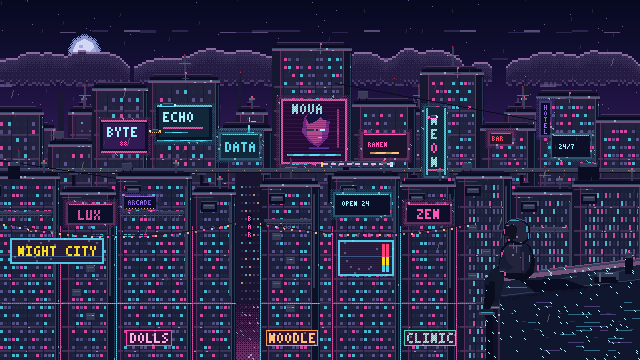
\includegraphics[width=0.78\textwidth]{figures/season_rain.png}
\caption{雨夜霓虹场景设计画面}
\end{figure}
雨夜以冷色天空与城市霓虹为主体，雨线穿过楼宇前景，路面反射霓虹光斑；建筑灯光与街区屏幕形成清晰的视觉焦点。

\begin{figure}[H]\centering
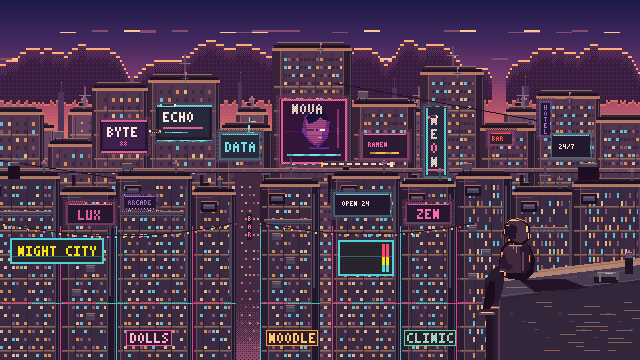
\includegraphics[width=0.78\textwidth]{figures/season_thunder.png}
\caption{黄昏雷云场景设计画面}
\end{figure}
黄昏场景保留夜城的空间布局，通过天空、楼体与灯光的暖色变化营造雷云来临的氛围，闪电不时照亮整座城市。

\begin{figure}[H]\centering
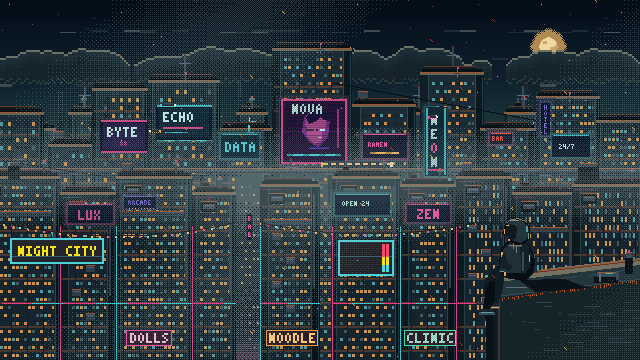
\includegraphics[width=0.78\textwidth]{figures/season_fog.png}
\caption{薄雾深夜场景设计画面}
\end{figure}
薄雾场景以柔和的灰绿层次突出城市纵深，雾带、窗光与前景人物共同组织静谧的夜间画面。

\begin{figure}[H]\centering
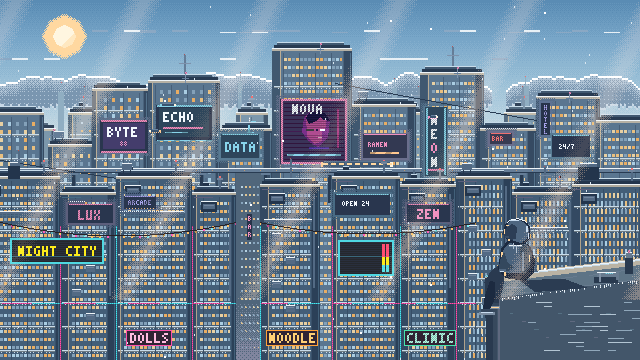
\includegraphics[width=0.78\textwidth]{figures/season_snow.png}
\caption{飘雪清晨场景设计画面}
\end{figure}
飘雪清晨以明亮的天空和冷色建筑为背景，雪粒飘落，屋顶积雪，人物呼出白气，延续统一的城市风格。

\paragraph{街区细节。}前景建筑配置 \texttt{NIGHT CITY} 显示屏、音乐显示屏、店铺招牌、轮廓灯带和悬挂灯串。扫描线、呼吸亮度及灯泡追逐由帧计数驱动；悬挂灯的下垂弧线以分段阈值近似，避免逐像素执行乘法。

\paragraph{场景进入与返回。}拨动 SW3 进入场景时，控制器先保存当前静图编号；场景模式下方向键在四季间切换。退出时，控制器等待静图事务排空并确认已恢复到保存的图片，再把画面交回静图通路；恢复期间仍显示场景，观众不会看到未准备好的背景。背景音乐、字幕和菜单在两种模式间共享，模式切换只改变显示内容。

\paragraph{显示完成令牌。}25 MHz 合成域生成一帧，不等于 HDMI 输出端已经送出这一帧。为此，输出侧维护带场景序号和代次的帧开始／完成令牌，控制侧只有收到匹配的令牌才确认场景已真正呈现；即使快速来回切换到同一场景编号，代次也能区分新旧事件，保证场景标题、字幕和实际画面严格对应。

\subsubsection{图层合成与 720p 输出模块}
\paragraph{图层顺序。}背景来自 SDRAM 静图或四季场景，依次经过转场增益与亮度／对比度调节、字幕与状态提示、音频柱、中文菜单各图层，最后进入 720p 扫描输出（图\ref{fig:layers}）。每个叠加层只在自己的坐标范围内覆盖像素，其余位置透传下层，所有图层共用一条像素流水，不需要额外帧缓存。

\begin{figure}[H]\centering
\begin{tikzpicture}[node distance=4mm,box/.style={draw,align=center,minimum width=3.6cm,minimum height=0.72cm,fill=blue!5},arr/.style={-{Latex},thick}]
\node[box] (a) {背景：缓存图／四季场景};
\node[box,below=of a] (b) {转场与亮度、对比度};
\node[box,below=of b] (c) {字幕与状态提示};
\node[box,below=of c] (c2) {音频幅度柱};
\node[box,below=of c2] (d) {中文菜单};
\node[box,below=of d] (e) {行缓存倍扫与 HDMI 输出};
\draw[arr](a)--(b); \draw[arr](b)--(c); \draw[arr](c)--(c2); \draw[arr](c2)--(d); \draw[arr](d)--(e);
\end{tikzpicture}
\caption{视频图层处理顺序}\label{fig:layers}
\end{figure}

\paragraph{亮度与对比度。}像素通路以定点运算实现
\begin{equation}
P'=\operatorname{clip}_{[0,255]}\!\left(C(P-P_0)+P_0+B\right),
\end{equation}
其中 $P$ 为输入颜色分量，$P_0$ 为中性参考，$C$、$B$ 分别为对比度与亮度控制量，结果饱和限幅到 8 位。菜单参数在帧起点取快照，保证同一帧内参数一致。

\paragraph{720p 倍扫输出。}所有内容在 $640\times360$ 画布上以 25 MHz 合成，再经扫描输出模块 \texttt{hd720\_composite\_scanout}（下表）在 74.25 MHz 像素域按 $1280\times720$@60 Hz 标准时序输出。画布坐标 $(x,y)$ 与输出坐标 $(X,Y)$ 的关系为
\begin{equation}
x=\left\lfloor X/2\right\rfloor,\qquad y=\left\lfloor Y/2\right\rfloor .
\end{equation}
合成域每产生一行像素，经像素 FIFO 跨入像素域，写入两个交替使用的行缓存；像素域每行读两遍、每像素重复两次，完成横纵各两倍放大。合成域只在行缓存有空位时才推进下一行，因此两个时钟域之间不需要整帧缓冲。复杂的场景与菜单逻辑留在 25 MHz 域，高频像素域只负责扫描与封装，这是设计能够时序收敛的关键。

\begin{figure}[H]\centering
\begin{tikzpicture}[node distance=8mm,box/.style={draw,align=center,minimum width=2.4cm,minimum height=0.8cm,fill=blue!5},arr/.style={-{Latex},thick}]
\node[box] (a) {$640\times360$\\图层合成}; \node[box,right=of a] (b) {跨域 FIFO\\及双行缓存}; \node[box,right=of b] (c) {横纵各 2 倍\\像素扫描}; \node[box,right=of c] (d) {720p60\\HDMI 发送};
\draw[arr](a)--(b); \draw[arr](b)--(c); \draw[arr](c)--(d);
\draw[arr,dashed](b.south)--++(0,-0.5)-|node[pos=0.25,below,font=\scriptsize]{行空位信用}(a.south);
\end{tikzpicture}
\caption{内部画布到 HDMI 输出的适配}\label{fig:720}
\end{figure}

\begin{center}\small
\begin{tabular}{>{\raggedright\arraybackslash\ttfamily\footnotesize}p{6.0cm}C{1.0cm}C{1.6cm}>{\raggedright\arraybackslash}p{4.7cm}}
\toprule
信号名 & 位宽 & 方向 & 功能描述\\\midrule
\tablegroup{source\_clk / pixel\_clk} & 1 & Input & 25 MHz 合成时钟与 74.25 MHz 像素时钟\\
\tablegroup{source\_vs / source\_de} & 1 & Input & 画布帧同步与有效像素\\
source\_rgb & 24 & Input & 合成后的画布像素\\
source\_frame\_tag & 32 & Input & 帧标签（场景序号与代次）\\
row\_free & 2 & Output & 两个行缓存的空位信用\\
\tablegroup{axis\_valid / axis\_data} & \tablegroup{1 / 24} & Output & 送往 HDMI 发送核的视频流\\
\tablegroup{axis\_user / axis\_last} & 1 & Output & 帧起点与行末标志\\
axis\_ready & 1 & Input & 发送核就绪\\
\tablegroup{frame\_start\_tag / frame\_done\_tag} & 32 & Output & 输出端帧开始与完成令牌\\
\bottomrule
\end{tabular}
\end{center}

\subsubsection{交互控制、字幕与转场模块}
\paragraph{输入事件路由。}按键与拨码开关先经三级同步和 20 ms 消抖，转换为单次事件，再由 \texttt{player\_menu\_control} 根据当前模式统一解释：同一方向键在菜单打开时用于选择和调整，菜单关闭时用于切图，场景模式下用于切换季节。任一时刻只有一条控制路径响应按键，避免一次按键同时改变菜单和画面。

\begin{center}\small
\begin{tabular}{p{2.0cm}p{10.8cm}}
\toprule
输入 & 功能\\\midrule
KEY1 & 系统复位，重新加载素材与默认状态\\
KEY2 & 菜单内进入或确认\\
\tablegroup{KEY3 / KEY4} & 菜单外切换\tablegroup{下一张 / 上一张}；菜单内选择或调整参数\\
SW1 & 开启或关闭静图自动轮播\\
SW2 & 打开或关闭中文菜单\\
SW3 & 进入或退出四季动态场景\\
\bottomrule
\end{tabular}
\end{center}

菜单分两级：一级选择亮度、音量、对比度、滚动字幕、音频可视化、轮播周期、图片选择和音乐选择八项功能，二级调整具体参数。菜单文字使用片上中文字库，当前曲目标题从 TF 卡读取后显示。

\paragraph{中文滚动字幕。}六幅静图各配一条中文说明，四季场景共用一条，共七条文案、214 个不同汉字。构建时只把实际用到的字形打包进片上 ROM，并为每条消息生成字符序列。字幕的选择由已呈现的图片编号或场景状态决定并在帧边界锁定，因此字幕总与屏幕上的内容一致；切换内容时字幕从起点重新滚动，菜单中可随时开关。

\paragraph{淡出—黑场—淡入转场。}\texttt{image\_fade\_transition} 以八状态机控制切图（图\ref{fig:fade-fsm}）：收到新帧就绪令牌后，增益 $\alpha$ 从 32 起每帧递减 3 至 0，旧图淡出；黑场期间切换读出缓存编号，等待旧读请求退出、新读请求获得应答；随后 $\alpha$ 每帧递增 3 回到 32，新图淡入，并返回呈现应答。输出像素为 $P_{\mathrm{out}}=\alpha P_{\mathrm{in}}/32$，淡出和淡入各约 11 帧。缓存切换发生在全黑画面中，观众看不到任何半帧或撕裂。

\begin{figure}[H]\centering
\begin{tikzpicture}[font=\scriptsize,st/.style={draw,thick,rounded corners,minimum width=1.55cm,minimum height=0.7cm,align=center,fill=blue!5},arr/.style={-{Latex},thick}]
\node[st] (idle) at (0,0) {IDLE};
\node[st] (start) at (2.4,0) {START};
\node[st] (out) at (4.8,0) {FADE\_OUT\\$\alpha\downarrow$};
\node[st] (quiet) at (7.2,0) {QUIET\\切换缓存};
\node[st] (req) at (7.2,-1.6) {REQUEST};
\node[st] (ack) at (4.8,-1.6) {ACK};
\node[st] (rev) at (2.4,-1.6) {REVEAL};
\node[st] (in) at (0,-1.6) {FADE\_IN\\$\alpha\uparrow$};
\draw[arr](idle)--node[above]{就绪令牌}(start); \draw[arr](start)--(out); \draw[arr](out)--node[above]{$\alpha=0$}(quiet);
\draw[arr](quiet)--node[right]{旧读退出}(req); \draw[arr](req)--node[above]{读请求}(ack); \draw[arr](ack)--node[above]{应答}(rev);
\draw[arr](rev)--(in); \draw[arr](in)--node[left]{$\alpha=32$，返回呈现}(idle);
\end{tikzpicture}
\caption{淡出淡入转场状态机}\label{fig:fade-fsm}
\end{figure}

\paragraph{自动轮播。}自动轮播提供 3、5、15 秒三档。控制器在新图完整呈现后才开始计时，以 25 MHz 计数，5 秒对应 $25\,000\,000\times5=125\,000\,000$ 个时钟周期；手动切图或模式变化会让计时重新开始，保证每张图都能完整停留设定的时长。

\subsubsection{设计取舍}
作品优先保证同一镜像中音画连续和多功能共存，在三个关键处做了取舍：
\begin{itemize}
\item \textbf{$640\times360$ 画布＋720p 输出}：复杂图层在 25 MHz 合成，像素域只做倍扫，在 EG4S20 的资源与时序条件下同时获得 720p 高清接口和丰富的叠加内容；画布与 16:9 显示器比例一致，无黑边浪费。
\item \textbf{六帧启动缓存}：启动时一次性加载全部图片，此后切图零读卡等待，并把 TF 卡带宽完整留给音乐播放。
\item \textbf{构建时字库}：只打包实际用到的 214 个汉字，在 RAM 已用满的器件上实现中文字幕和中文菜单。
\end{itemize}

\subsubsection{功能验证方法与结果}
设计采用“模块仿真—布局布线—上板运行”三级验证：模块仿真用独立参考模型逐像素比对 RTL 输出，检查像素、状态和接口；布局布线检查资源与时序；上板运行检验图像、声音与交互在同一镜像中的协同效果。

\begin{center}\small
\begin{tabular}{p{3.0cm}p{6.6cm}p{3.6cm}}
\toprule
验证对象 & 验证方法 & 结果\\\midrule
图片缩放 & $640\times480$ 输入经缩放模型与 RTL 对比 $640\times360$ 画布全部 230400 像素 & 内容区 $480\times360$，最大通道偏差 1\\
四季场景 & 28 帧 RTL 输出与独立模型逐像素比较，并检查天气变化与音频柱历史 & 逐像素一致\\
中文字幕 & 核对七条文案、214 个字形像素、帧边界选择与叠加 & 全部通过\\
场景 ROM & 从生成数据独立重建 13 块 ROM 内容，与网表中的初始化值逐块比对 & 全部一致\\
时序收敛 & TD 布局布线时序报告 & 全部时钟域无违例\\
整机运行 & 同一固化镜像上板，逐项操作基础与扩展功能 & 全部功能正常\\
固化启动 & 写入 Flash 并自动校验，断电后重新上电 & 自动启动，图音正常\\
\bottomrule
\end{tabular}
\end{center}

\section{完成情况及性能参数}

\subsection{整体介绍}
作品已形成由开发板、TF 卡和 HDMI 显示器组成的完整多媒体展示系统。基础功能、五类拓展功能与四季动态场景集成在同一固化镜像中，全部功能均在实物上正常运行。镜像写入配置 Flash 后，断电再上电，画面与声音自动启动，无需连接电脑。

\photoplaceholder{系统正面整体展示}{使开发板、TF 卡槽、HDMI 连接和显示器同框；屏幕显示作品的四季夜城或静图，保持画面清晰，避免拍入身份信息。}
\photoplaceholder{系统斜向整体展示}{从约 45 度拍摄设备布局与线缆连接，保证开发板与显示内容同时可辨，不遮挡板载按键。}

\subsection{工程成果}

\subsubsection{硬件成果}
系统使用 HX4S20C 板载资源构成 FPGA、TF、SDRAM、配置 Flash 和 HDMI 接口。图片和音乐从 TF 卡进入 FPGA，图像经 SDRAM 缓存后与动态场景及各图层合成，经 HDMI 同时送出画面与声音。全部运行时处理在 FPGA 内完成，无需外接处理器。

\photoplaceholder{开发板与接口实物}{近距离拍摄开发板正面，使芯片、TF 卡槽、HDMI 输出、按键与拨码开关的位置清楚可见。}

\subsubsection{FPGA 逻辑成果}
FPGA 逻辑涵盖 TF 卡访问与素材解析、双线性缩放、六帧缓存与刷新调度、音频播放与音量处理、图层合成、中文菜单与字幕、四季场景生成和 720p 音视频输出，在 EG4S20 上完成综合、布局布线并全部时序收敛。

\photoplaceholder{工程工具与构建结果界面}{在 TD 工程工具中显示当前作品的器件、主要资源或布局布线结果，截图时保留可辨读的结果区域，裁去本机用户名、路径和与作品无关的信息。}

\begin{center}\small
\begin{tabular}{p{4.6cm}p{2.4cm}p{2.4cm}p{3.2cm}}
\toprule
资源 & 使用 & 器件容量 & 利用率\\\midrule
LUT & 16454 & 19600 & 84.0\%\\
寄存器 & 9007 & 19600 & 46.0\%\\
SLICE & 8533 & 9800 & 87.1\%\\
9 Kb RAM 块 & 63 & 64 & 98.4\%\\
32 Kb RAM 块 & 16 & 16 & 100\%\\
DSP & 24 & 29 & 82.8\%\\
PLL & 4 & 4 & 100\%\\
\bottomrule
\end{tabular}
\end{center}
片上 RAM 与 PLL 全部用满、LUT 利用率达 84\%，说明作品充分挖掘了 EG4S20 的硬件资源；在如此高的利用率下全部时钟域仍然时序收敛，setup 最差余量 $+0.682$ ns，保证了系统长期稳定运行。

\subsection{特性成果}
\subsubsection{基础功能与扩展功能总览}
\begin{center}\small
\begin{tabular}{p{2.8cm}>{\raggedright\arraybackslash}p{7.4cm}p{3.0cm}}
\toprule
功能 & 作品实现 & 完成情况\\\midrule
图片播放 & TF 卡读取 24 位 BMP，经 SDRAM 缓存后 HDMI 720p 输出 & 已完成，实物运行正常\\
手动与自动切图 & 按键前后切换；拨码开启自动轮播，周期 \tablegroup{3 / 5 / 15} 秒可选 & 已完成，实物运行正常\\
音频播放 & 48 kHz 立体声 PCM，HDMI 音频输出，四首曲目菜单选择 & 已完成，实物运行正常\\
固化启动 & 统一镜像写入 Flash，上电自动加载运行 & 已完成，实物运行正常\\
文字叠加 & 七条中文字幕随\tablegroup{图片 / 场景}切换并滚动显示 & 已完成，实物运行正常\\
图像转场 & 旧画面淡出至黑、新画面淡入 & 已完成，实物运行正常\\
不同尺寸缩放 & BMP 几何解析、等比双线性缩放与居中补黑 & 已完成，实物运行正常\\
实时参数调节 & 中文菜单调节亮度、对比度、音量、字幕、轮播等 & 已完成，实物运行正常\\
音频可视化 & 真实 PCM 驱动主画面 64 柱与街区 12 柱音乐屏 & 已完成，实物运行正常\\
四季动态场景 & 四景切换、天气灯光实时变化、无缝返回静图 & 已完成，实物运行正常\\
\bottomrule
\end{tabular}
\end{center}

\subsubsection{图片读取、缩放与轮播}
系统配置六幅展示图，包括腕表、饮品、芯片、暴雨提示、车道提示及课堂展示。其中芯片图为 $640\times480$、24 位 BMP，系统自动等比缩放到 $480\times360$ 内容区并在两侧补黑，原图比例完整保留；其他尺寸的图片由同一套几何规则自动适配。按键切图与自动轮播都伴随淡出淡入转场，背景音乐持续播放。

\photoplaceholder{图片显示与比例适配实物}{拍摄芯片图完整画面及其左右黑边；另拍一幅宽画面素材，能看出显示区域与原始长宽比的关系。}
\photoplaceholder{手动切图与自动轮播实物}{分别拍摄操作按键／拨码与切换前后的画面，若需说明转场过程，可从实拍视频中选取淡出、黑场和淡入三帧。}

\subsubsection{中文菜单与实时参数}
拨动 SW2 打开中文菜单，方向键选择功能，确认键进入调整；调整结果立即作用于画面或声音。亮度和对比度改变背景像素，音量同时改变声音和音频柱高度，观众可直接观察控制量与效果的对应关系。

\photoplaceholder{中文菜单与参数调节实物}{拍摄一级菜单、一个二级参数页及调整前后画面，保证参数文字和背景可同时辨认；必要时分别放置两张照片。}

\subsubsection{滚动字幕与图像转场}
每幅静图和四季场景都有对应的中文字幕，切换内容时字幕同步更新并重新滚动，可在菜单中开关。切图时旧画面平滑淡出到黑，再淡入新图，过渡自然流畅。

\photoplaceholder{中文字幕与转场实物}{拍摄字幕清晰可读的两幅不同画面；转场可用连续实拍帧展示旧图、黑场与新图，勿用后期效果替代设备输出。}

\subsubsection{音频播放与音频可视化}
系统播放 48 kHz 立体声音乐，可在菜单中选择四首曲目。主画面底部 64 根幅度柱随音乐节奏起伏滚动，夜城街区的音乐屏同步跳动；调节音量时，声音与柱高一同变化。

\photoplaceholder{选曲与音频可视化实物}{画面同时包含曲目菜单或播放画面与音频柱；可另外拍摄静音和恢复音量两个状态，并通过实录声音保存听音证据。}

\subsubsection{四季动态夜城}
拨动 SW3 进入动态场景，方向键在雨夜霓虹、黄昏雷云、薄雾深夜和飘雪清晨之间切换。同一座城市在四季中呈现截然不同的色彩与天气：雨线、闪电、雾带、雪粒持续运动，霓虹招牌呼吸闪烁，街区音乐屏随音乐跳动。再次拨动 SW3 即回到原静态图片，音乐全程不中断。

\photoplaceholder{四季动态场景实物组图}{以相同机位分别拍摄四种场景；每张图保留清晰的屏幕边界，画面能区分雨、云、雾和雪的视觉变化。}
\photoplaceholder{街区细节与音乐联动实物}{近拍 NIGHT CITY 广告屏、店铺招牌、灯带及音频小屏；以视频或不同时间的实拍帧记录动态变化。}

\subsubsection{仿真验证结果}
四季场景的 28 帧 RTL 输出与独立参考模型逐像素一致，天气变化和音频柱历史符合设计；字幕验证覆盖全部七条文案和 214 个字形；$640\times480$ 输入的缩放结果在全部 230400 个画布像素上与模型的最大通道偏差仅为 1。仿真、布局布线和实物运行三级验证共同确认了设计的正确性。

\subsubsection{固化与上电运行}
最终镜像写入配置 Flash 并通过自动校验。断电后重新上电，无需重新下载或按复位键，系统自动完成素材加载，画面与声音正常启动，全部功能均可在该镜像上直接使用。

\photoplaceholder{固化上电后的运行实物}{拍摄上电运行的开发板与显示器；保留不连接下载电脑的正常使用画面，条件允许时用连续视频补充断电、上电与启动过程。}

\section{总结}

\subsection{作品成果}
本作品在一块安路 EG4S20 FPGA 开发板上，实现了一台功能完整、即插即用的数字艺术多媒体画框：
\begin{itemize}
\item \textbf{功能全面}：赛题的全部基础要求与五类拓展功能均已实现，并额外打造了四季动态夜城这一特色展示内容；
\item \textbf{一镜到底}：所有功能集成在同一个固化镜像中，插上 TF 卡、接上显示器、通电即可运行，现场无需电脑和任何调试操作；
\item \textbf{音画一体}：图片、音乐、字幕、转场与动态场景同时工作，切换内容时音乐不断、画面不闪；
\item \textbf{操作简单}：四个按键和三个拨码开关配合中文菜单，即可完成切图、选曲、调节画面和切换场景，普通观众无需说明书也能上手。
\end{itemize}

\subsection{应用效果}
作品把静态图片、背景音乐和随时间变化的数字艺术画面融为一体，观众既能看到清晰的图片内容和中文说明，又能感受到画面随音乐跳动、随季节变换的动态氛围。这种“图片＋音乐＋动态艺术”的组合，使原本单调的信息屏变成具有观赏性的展示终端，更容易吸引观众驻足。

作品不依赖网络、不需要上位机，只要准备好 TF 卡中的图片和音乐即可长期离线运行；更换展示内容时只需替换卡中素材，现场人员无需任何专业知识。基于 FPGA 的纯硬件实现上电即用、运行稳定，适合长时间无人值守的展示环境。

\subsection{应用前景}
\begin{itemize}
\item \textbf{展厅与博物馆}：展品图片配合中文字幕讲解与背景音乐，空闲时以动态夜城营造艺术氛围，提升参观体验；
\item \textbf{商业空间与橱窗}：自动轮播产品图片，动态场景作为吸引视线的数字艺术背景，营造独特的品牌氛围；
\item \textbf{校园与公共信息屏}：轮播通知与安全提示，更新内容只需替换 TF 卡，部署与维护成本低；
\item \textbf{家居数字画框}：播放家庭照片与喜爱的音乐，四季场景提供随时间变化的装饰画面，让墙面“活”起来；
\item \textbf{教学演示}：作为 FPGA 多媒体处理的完整实例，直观展示数字电路如何同时处理图像、声音与交互。
\end{itemize}

\subsection{可扩展之处}
作品采用模块化设计，各部分接口清晰，便于进一步扩展：可以增加新的场景主题，例如节日或城市地标风格；可以更换字幕文案以适配不同展示内容；还可以接入更大的存储或更高的显示分辨率，以容纳更多图片和更精细的画面。新功能可沿用现有的场景控制、图层合成与交互框架，扩展成本较低。

\subsection{作品总结}
本作品以“赛博美学数字艺术多媒体交互画框”为主题，完整实现了赛题要求的 HDMI 多媒体播放系统，并以四季动态夜城展现了 FPGA 在实时数字艺术方面的潜力。全部功能在一块开发板、一个固化镜像中协同运行，开机即用、操作直观。作品表明，仅凭一颗国产 FPGA 芯片，就能构建一台兼具实用性与观赏性的离线音画展示终端，为展陈、商业、校园和家居等场景提供一套完整、可落地的解决方案。

\section{参考文献}
\begin{enumerate}[label={[\arabic*]}]
\item 全国大学生嵌入式芯片与系统设计竞赛 FPGA 创新设计赛道．选题指南：基于安路 EG4S20 的 HDMI 多媒体播放系统[Z]．2026.
\item 安路科技．赛题解析一：基于安路 EG4S20 的 HDMI 多媒体播放系统[Z]．2026.
\item 安路科技．HX4S20 系列 FPGA 开发板使用手册[Z]．
\item 安路科技．TD 6.2.1 开发工具与 EG4S20 器件相关技术资料[Z]．
\item GNU Project．GNU Unifont 18.0.01 字体（SIL Open Font License 1.1）[EB/OL]．
\item Video Stream Scaler．流式视频缩放核（GNU LGPL-2.1-or-later）[EB/OL]．
\item 本作品工程．双线性流式缩放核、厂商 IP 和素材来源及许可记录[Z]．
\item HDMI Licensing, LLC．High-Definition Multimedia Interface Specification Version 1.4b[S]．2011.
\end{enumerate}


\end{document}
